
\documentclass[12pt ]{iopart}
\usepackage{graphicx}
\usepackage{amsmath}
\usepackage[space]{grffile}
\usepackage{epstopdf}
\usepackage[autostyle,italian=guillemets]{csquotes}%bibliografia
%%\usepackage[bibstyle=authoryear,citestyle=authoryear-comp,backend=biber,uniquelist=false]{biblatex}%stile bibliografia
\usepackage[style=authoryear-icomp,maxbibnames=9,maxcitenames=1,uniquelist=false,
    backend=biber]{biblatex}

\usepackage{algorithm}
\usepackage[noend]{algpseudocode}

\addbibresource{b.bib}
%\newcommand{\gguide}{{\it Preparing graphics for IOP Publishing journals}}
%Uncomment next line if AMS fonts required
%\usepackage{iopams}  
\begin{document}

\title[DNN for EEG-fNIRS BCI]{Deep Learning for  hybrid EEG-fNIRS Brain Computer Interface: application to Motor Imagery Classification}

\author{Pierpaolo Croce\textsuperscript{1,2}, Filippo Zappasodi\textsuperscript{1,2}, Francesco di Pompeo\textsuperscript{1,2} Arcangelo Merla\textsuperscript{1,2} \& Antonio Maria Chiarelli\textsuperscript{1,2}}

\ead{pierpaolo.croce@unich.it}
\vspace{10pt}
\begin{indented}
\item[] \textsuperscript{1} Department of Neuroscience, Imaging and Clinical Sciences, "G.d’Annunzio" University, Chieti, Italy
\item[] \textsuperscript{2} Institute of Advanced Biomedical Technologies, "G.d’Annunzio" University, Chieti, Italy
\end{indented}

\begin{abstract}
	\\
	\textit{Objective.} to be filled. \\
	\textit{Approach.} to be filled.\\
	\textit{Main Results.} to be filled. \\
	\textit{Significance.} to be filled.
\end{abstract}


\section{Introduction}

Brain Computer Interface (BCI) refers to a group of procedures that directly link  central nervous system to a computer or a device [ref.]. BCI can focus on mapping, assisting, augmenting, or repairing human cognitive and sensory-motor functions. 
Historically, BCI was performed using Electroencephalography (EEG) [ref.]. EEG  provides information regarding brain electrical activity with very high temporal resolution (ms scale) [ref.]. 

In the last years, BCI studies investigated the possibility of combining EEG with other neuroimaging technologies [ref.]. Among these, functional Near Infrared Spectroscopy (fNIRS) provided encouraging results [ref.]. 

EEG and fNIRS are both flexible, scalp located procedures. Whereas EEG captures the macroscopic temporal dynamics of brain electrical activity through passive voltages evaluation, fNIRS estimates brain hemodynamic oscillations  relying on spectroscopic measurements of oxy- and deoxy-hemoglobin (HbO and Hb, respectively) fluctuations in the cortex [ref.]. Orthogonally with respect to EEG, fNIRS, depending on the slow dynamics of the hemodynamic response, yields low temporal resolution but, because of the fast exponential decay of light sensitivity, it provides good spatial resolution (around 1 cm) \parencite{chiarelli2016combining}. 

Because of different physiological information provided by and characteristic of EEG and fNIRS [ref. croce], higher BCI performances  of combined measurements with respect to standalone EEG were reported extensively [ref.] .

Two main processing steps are involved in BCI:  feature extraction and classification. 

EEG features are usually extracted based on the power of the signal frequency bands. Indeed, well-distinct behaviors of EEG signal have been identified based on signal frequencies (delta ($< 4 Hz$), theta ($4-7 Hz$), alpha ($8-15 Hz$), beta ($16-31 Hz$), and gamma ($> 31 Hz$) ref.]). For example, during the execution of a motor task (or during the imagination or observation of the movement), the beta activity is suppressed in related brain areas(Event Related Desynchronization, ERD)[ref.].  
fNIRS  features are generally  computed from  HbO and Hb variations in the brain which are dependent, among others, on the  Blood Oxygen Level Dependant (BOLD) effect [cit.]. 

The classification procedure aims to accurately classify the brain state  based on the extracted signal features  and it is a fundamental step of BCI processing.


Different  experiment and algorithms have been applied  to combined EEG-fNIRS BCI. \textcite{Fazli_2012} proposed Linear Discriminant Analysis to classify ERD EEG and time average fNIRS concentration changes during executed movements as well as motor imagery.  In \textcite{ma2012hybrid} a Gaussian radial-basis kernel Support Vector Machine (SVM) was used to classify a motor imagery BCI based on EEG power spectral densities and fNIRS amplitude of the cerebral blood oxygen signal.   \textcite{lee2014hybrid} employed LDA on combined EEG and fNIRS features to classify three conditions: right and left motor imagery and idle status . They reached a classification accuracy of about $65\%$. In \textcite{buccino2016hybrid} the features to be submitted to a LDA were extracted combining two methods: Regularized Common Spatial Patterns (RCSP) for EEG and combination of average and slope indicators for fNIRS signals. In this case an accuracy between $72-79\%$ was reached in a movement recognition task. In  \textcite{khan2014decoding, khan2017hybrid} LDA was used to classify control commands based on EEG peak amplitudes of selected motor area channels and mean values of HbO and Hb for fNIRS with accuracy ranging between $80-95\%$.
For all of the above mentioned studies, the authors recognized and increase BCI performance of combined measurements with respect to standalone fNIRS and EEG.

Recently, Deep Learning Classifiers are increasing their popularity. In the simplest fashion, Deep Learning  refers to Artificial Neural Networks (NN) [ref.] that are composed of many layers. Deep NNs (DNN) use a cascade of  layers of nonlinear processing units (neurons). Each successive layer uses the output from the previous layer as input and all, or part, of the neurons from consecutive layers are connected. DNN can perform very complex, non-linear, transformations-classifications, greatly increasing shallow NN  [cit.]  and other classifiers performances (LDA, SVM, etc.). In fact, they can reach unprecedented classification outcomes when applied to signals and or images [ref.]. Because of their performances, these algorithms are also receiving  attention within the biomedical field [cit.]. 
Multiple technological development allowed for Deep learning evolution. 
Among them, the increased computation power clearly played an important role.
However, the major improvements are algorithms related and they can be divided in three  categories:

\begin{itemize}
	\item[-] Implementation of Efficient learning algorithms that avoid local minima in the objective function and poor generalization (over-fitting) [ref.]; because of the presence of many free parameters (sometimes millions or more), and the possibility to represent very complex functions, DNN were usually affected by local minima in the objective function and over-fitting  during training. 
	\item[-] Development of new Neuron's activation functions (such as Rectified Linear Unit Function, ReLU function) that dampen  the vanishing gradient problem; in fact traditional activation functions such as the hyperbolic tangent or the sigmoid functions had wide ranges of the independent variables with small gradients;  this aspect, combined with the back propagation algorithm, exponentially dampened weight update rate going from the last to the first layers, heavily slowing the overall learning rate of the network.
	\item[-] Implementation of  Neural Networks were Neurons are connected to portions of signals and or images that are close in time and/or space (Convolutional Neural Networks, CNNs), encoding temporal and/or spatial information; standard, full connected DNN  did not encode any spatio-temporal information.
\end{itemize}

DNN have been successfully applied to  both EEG and fNIRS BCI classification problem. In \textcite{jirayucharoensak2014eeg} a Deep Learning Network was used to classify three levels of valence and arousal based on EEG power spectral densities  features. They reached an accuracy of about $50\%$. 
\textcite{hajinoroozi2015feature} employed Deep Belief Network to EEG signals for the classification of driver's cognitive states. 
In \textcite{an2014deep} left vs. right motor imagery classification  was performed by employing few EEG recording channels via DNN with an average accuracy of about $80\%$ . 
 \textcite{bashivan2015learning} trained a CNN using EEG power in three different frequency bands of interest. They reported a best-performance accuracy of about $92\%$.

Regarding fNIRS,only  few  studies were performed employing Deep Learning.  \textcite{hennrich2015investigating} investigated DNN classification performances of three mental task reporting accuracy values similar  to other classification algorithms (such as LDA and SVM).  \textcite{abibullaev2011neural} classified four mental task through DNN with an accuracy of $94\%$. Finally, \textcite{nguyen2013temporal} classified Left vs. Right motor imagery fNIRS activity with average accuracy of $85\%$. To the best of our knowledge, no studies implementing deep learning algorithm for BCI classifications  in a combined EEG-fNIRS framework were performed.

 In this paper, by expecting significant overall BCI performances,  we investigated the capabilities of combining multi modal EEG-fNIRS brain recordings  with state-of the art Deep learning Classification procedures. As a first investigation step, we performed a Left vs. Right Hand Motor Imagery task [cit.] and, by employing a common temporal frame of 1 second between technologies [cit.], Left vs Right classification accuracy of a DNN in in the multimodal recording modality  [ref.] was estimated and compared to other classification algorithms and to standalone EEG and fNIRS. 


\section{Methods}
\subsection{Experimental Paradigm}
Six healthy subjects (all -males, mean age of $34 \pm 5$ years) were recruited for the study. All subjects were right handed, as assessed by the Edinburgh questionnaire (PUNTEGGIO??, Oldifield 1971), reported no history of neurological or psychiatric disease and did not receive psychoactive medications. 
The subjects were seated in a chair at a desk and were asked to perform alternating squeezing motor imagery of right and left hand starting after an acoustic stimulus as depicted in the figure \ref{fig:fig2}. Motor imagery was performed for 5 seconds after the acoustic stimulus onset and was preceded and followed by 10 seconds of resting state. The subjects were instructed to perform the motor imagery with a frequency of repetition of about $1Hz$. The total number of trials was 20 for right and left motor imagery, respectively. 



\begin{equation}
	\begin{bmatrix}
		O_2Hb\\
		HHb
	\end{bmatrix}
	=
	\frac{1}{\rho}\begin{bmatrix}
		\epsilon_{O_2}(\lambda_1)\cdot DFP(\lambda_1)&\epsilon_{HHb}(\lambda_1)\cdot DFP(\lambda_1)\\
		\epsilon_{O_2}(\lambda_2)\cdot DFP(\lambda_2)&\epsilon_{HHb}(\lambda_2)\cdot DFP(\lambda_2)
	\end{bmatrix}^{-1}\times
	\begin{bmatrix}
	OD(\lambda_1)&\\
	OD(\lambda_2)
	\end{bmatrix}
	.
\end{equation}


\begin{equation}
\begin{bmatrix}
\Delta O_2Hb\\
\Delta HHb
\end{bmatrix}
=
\begin{bmatrix}
O_2Hb_{MI}-O_2Hb_{Bas}\\
HHb_{MI}-HHb_{Bas}
\end{bmatrix}
.
\end{equation}



\begin{equation}
\begin{bmatrix}
\Delta O_2Hb\\
\Delta HHb
\end{bmatrix}
=
\begin{bmatrix}
O_2Hb_{MI}-O_2Hb_{Bas}\\
HHb_{MI}-HHb_{Bas}
\end{bmatrix}
.
\end{equation}

\begin{equation}
y= 
\begin{cases}
0,& \text{if } wx+b \leq 0\\
wx+b,&\text{if } wx+b > 0
\end{cases}
\end{equation}

\begin{equation}
\begin{bmatrix}
P_{Right}\\
P_{Left}
\end{bmatrix}
=
\begin{bmatrix}
\frac{e^{x^Tw_1}}{\sum\limits_{k=1}^2 e^{x^Tw_k}}\\
\frac{e^{x^Tw_2}}{\sum\limits_{k=1}^2 e^{x^Tw_k}}
\end{bmatrix}
.
\end{equation}

\begin{equation}
cross entropy= 
-\sum\ y'\ln y
\end{equation}

\begin{figure}
	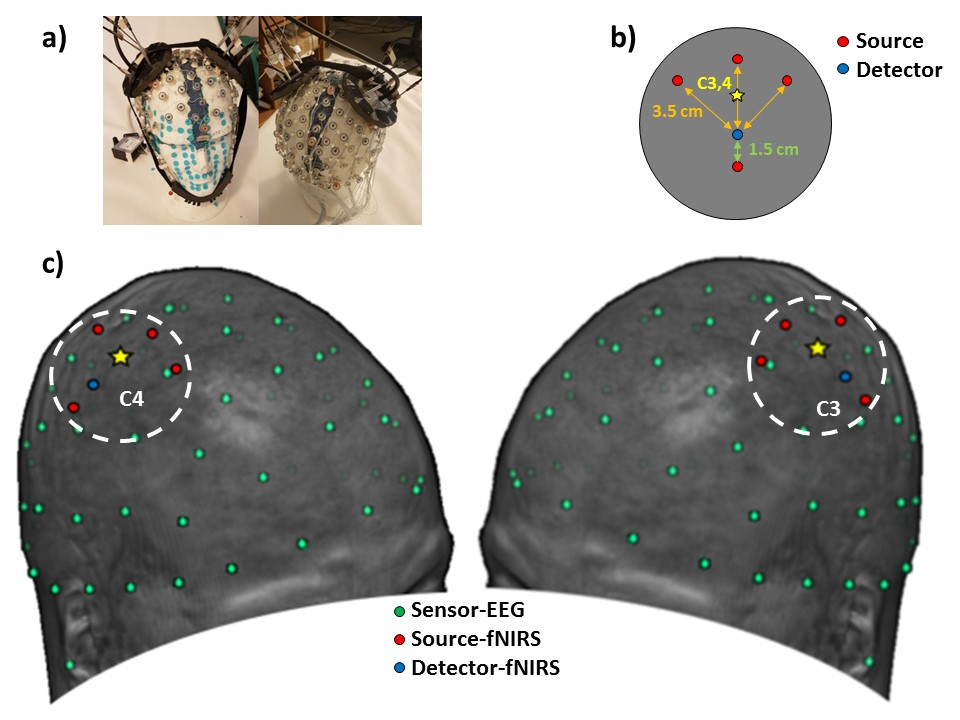
\includegraphics[width=\linewidth]{Diapositiva1.JPG}
	\caption{}
	\label{fig:fig1}
\end{figure}

\subsection{ElectroEncephalography Recordings}
Brain electric activity was recorded by a 128 channels EEG system (Electrical Geodesic Inc, EEG System Net 300).
Skin/electrode impedance was measured before each EEG recording and kept below 50 kΩ. EEG data were sampled at 250 Hz and processed on-line. For each subject and for each time window of 1 second during the task (5 seconds in total), data were filtered between 13 and 30 Hz (Butterworth filter of 2nd order, forward and back filtering). The filtered signal was then squared
and the time course of power modulation was evaluated (for each windows of 1 second) by calculating relative changes in power during the motor imagery execution (pMI) with respect to the mean power in a baseline period of 2 s prior to the onset (pMIBas). To this aim, Event-Related Synchronization (ERS) or Event-Related Desynchronization (ERD) (Pfurtscheller and Lopes da Silva, 1999; Neuper and Pfurtscheller, 2001) values were obtained according to:

\begin{equation}
\label{eqn:erders}
ERD/ERS=\frac{pMI-pMIBas}{pMIBas}100
\end{equation} 

Such ERD/ERS value were used as features for the learning algorithms used in the study. 
 
%EEG setup, online filtering (1 sec), differential power calculation, 

\begin{figure}
	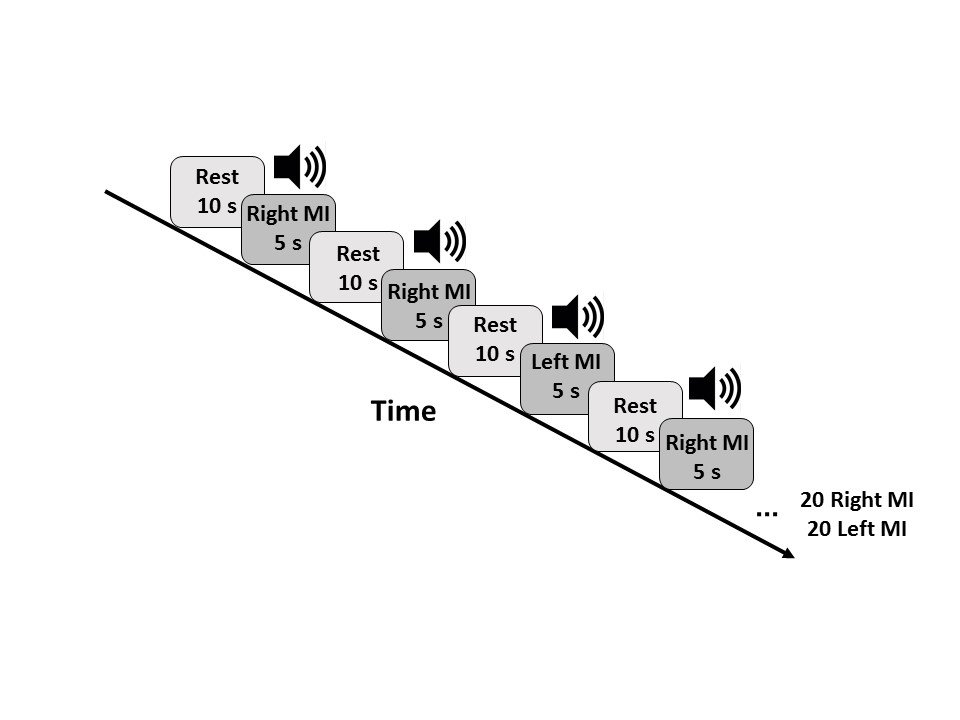
\includegraphics[width=\linewidth]{Diapositiva2.JPG}
	\caption{}
	\label{fig:fig2}
\end{figure}

\subsection{functional Near Infared Spectroscopy Recordings}
fNIRS setup, online hemoglobin evaluation, differential averaging (1 sec).
\subsection{Deep Neural Networks}
Introduction, layer structure,initialization, transfer functions, objective function, learning algorithm,  iterations, cross-validation,  accuracy, software Tensorflow
\begin{figure}
	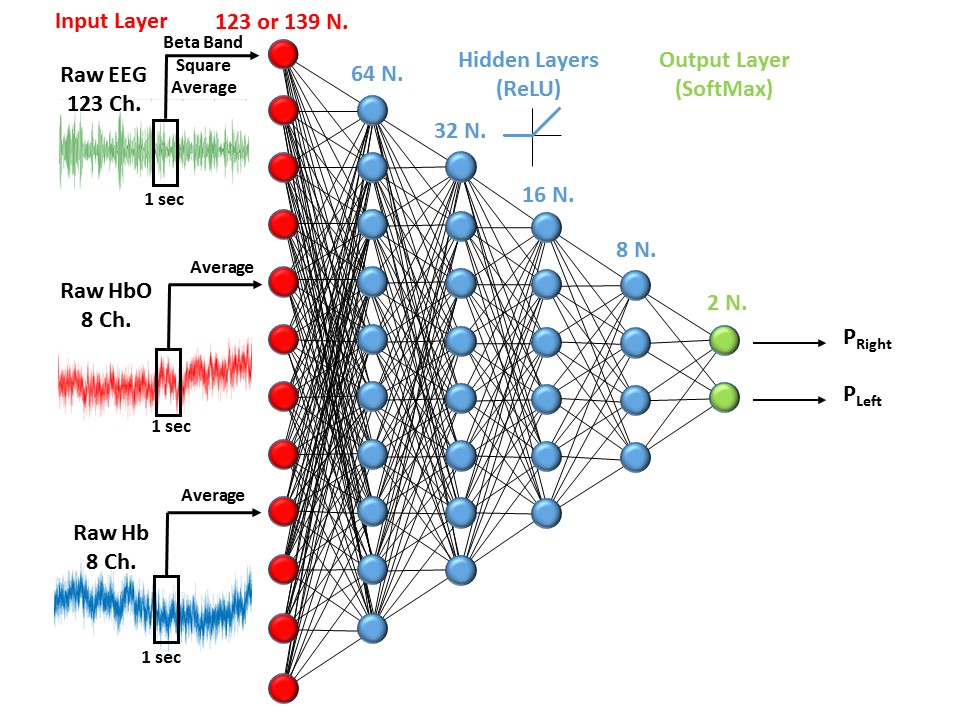
\includegraphics[width=\linewidth]{Diapositiva3.JPG}
	\caption{}
	\label{fig:fig3}
\end{figure}
\subsection{Post Processing and Statistical Analysis}
Brief introduction of LDA and SVM.
Two way anova recordings-classification.


\subsection{}
\section{Results}
The ERD/ERS time course of beta power for a representative subject is depicted in figure \ref{fig:fig4}b.
Example of average maps-timecourses.
Example of learning curve.
Best performance for DNN
Report overall Performances.
Two way anova SVM DNN of accuracy with respect to EEG-LDA.
Post hoc comparisons.
\begin{figure}
	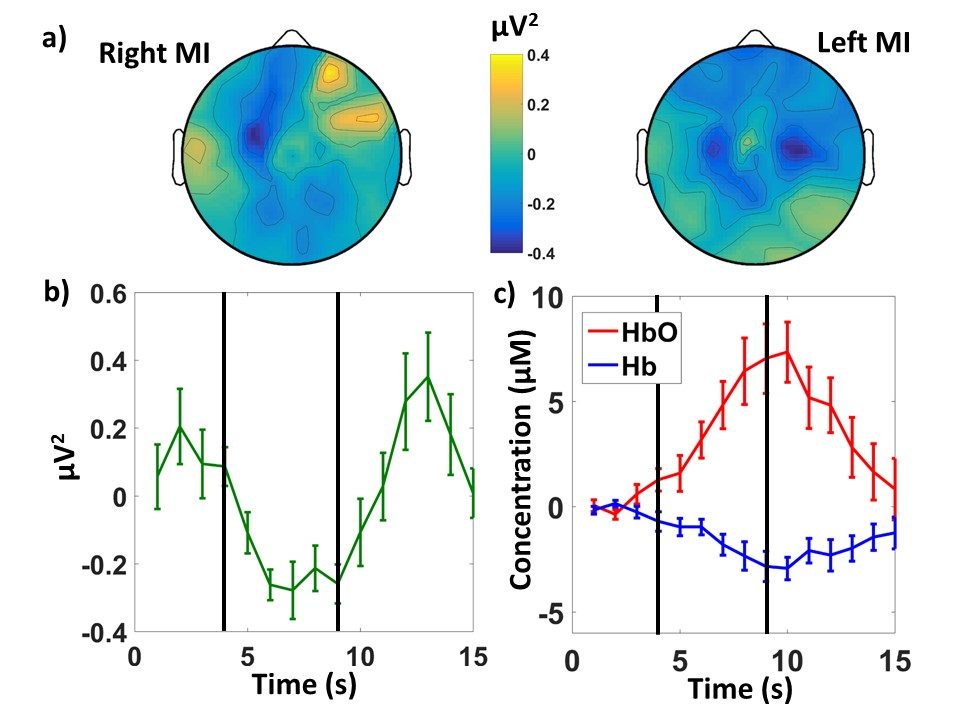
\includegraphics[width=\linewidth]{Diapositiva4.JPG}
	\caption{}
	\label{fig:fig4}
\end{figure}
\begin{figure}
	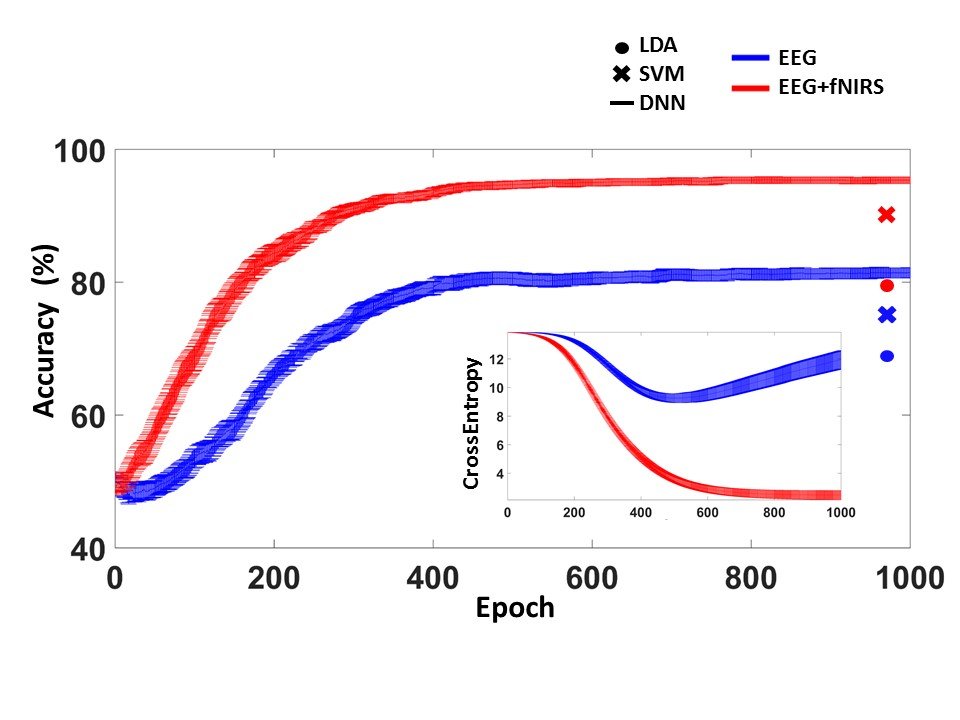
\includegraphics[width=\linewidth]{Diapositiva5.JPG}
	\caption{}
	\label{fig:fig5}
\end{figure}
\begin{figure}
	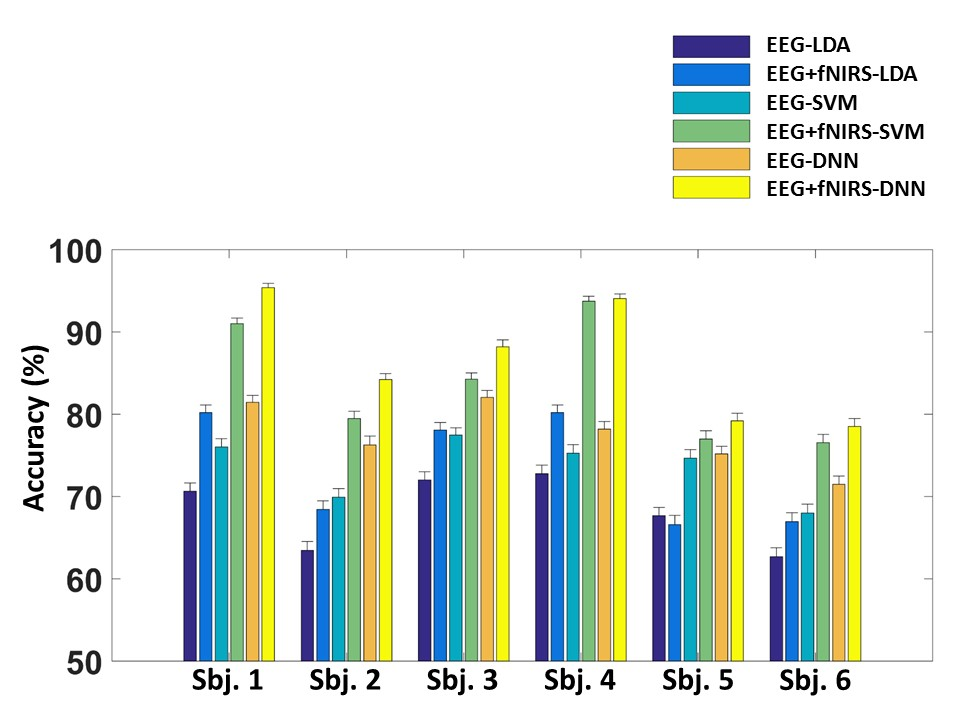
\includegraphics[width=\linewidth]{Diapositiva6.JPG}
	\caption{}
	\label{fig:fig6}
\end{figure}
\section{Discussion}
Short re-caption of main DNN concepts and EEG-fNIRS for MI.
Discussion of obtained results:
increased performance with fNIRS and with DNN classification without interaction (cumulative effect).
Limitations: fixed hyperparameters
(overall length of experiment, frequency band, response time (1sec), DNN structure). 
Report CNN results were poorer (low spatial information content of EEG), may work better with full-head fNIRS.






\section{Conclusion}

\section{Acknowledgements}
This study was partially funded by grant: H2020, ECSEL-04-2015-Smart Health, Advancing Smart Optical Imaging and Sensing for Health (ASTONISH).
 


\end{document}
\newpage
\printbibliography
%\cleardoublepage
%\addcontentsline{toc}{section}{\refname}